\documentclass{article}
\usepackage{listings,color,parskip,booktabs,longtable,array,
hyperref,multirow,multicol,enumitem}
\usepackage[top=1.1in, bottom=1.1in, left=1in, right=1in]{geometry}
\hypersetup{colorlinks,urlcolor=blue}
\lstset{frame=none,
	language=[LaTeX]{TeX},
  aboveskip=3mm,
  belowskip=3mm,
  showstringspaces=false,
  columns=flexible,
  basicstyle={\ttfamily},
  numbers=none,
  numberstyle=\tiny\color{gray},
  stringstyle=\color{mauve},
  breaklines=true,
  breakatwhitespace=true,
  tabsize=1
}
\usepackage{microtype,graphicx,amsmath,amssymb,float}
\usepackage[backend=bibtex]{biblatex}
\addbibresource{luamodular}
\begin{document}
\title{The luamodulartables Package in LaTeX}
\author{Chetan Shirore and Dr. Ajit Kumar}
\maketitle
\section{Introduction}\label{section:introduction}
The \verb|luamodulartables| package is developed to generate modular addition and multiplication tables for positive integers. It provides an easy way to generate modular addition and modular multiplication tables for positive integers in LaTeX documents. The commands in the package have optional arguments for the formatting of tables. These commands can be used in an environment similar to a  \verb|tabular| or \verb|array| environment. The commands can also be used with the \verb|booktabs| package, which provides nice formatting of tables in LaTeX. It is written in Lua, and TeX file is to be compiled with LuaLaTeX engine.


The Lua \cite{online.luaorg} programming language is a scripting language that can be embedded across platforms. With\verb|LuaTeX| \cite{online.luatex}  and\verb|luacode| \cite{online.luacode} packages, it is possible to use Lua in LaTeX. The TeX  \cite{online.tex} or LaTeX has scope for programming \cite{online.texscript}. However, with the weird internals of TeX, there are several limitations, especially for performing calculations on numbers in LaTeX documents. There are packages like \emph{pgf} \cite{online.pgf} and  \emph{xparse}  \cite{online.xparse} in LaTeX which provides some programming capabilities inside LaTeX documents. However, such packages do not provide the complete programming structure that Lua programming languages provide. The \verb|luacode| \cite{online.luacode}  package is used in its development apart from the \verb|luacode| package. The time required to generate modulo addition and multiplication tables is not an issue while compiling with LuaLaTeX. There is no need to install Lua on users system as TeX distributions (TeXLive or MikTeX) come bundled with LuaLaTeX. The package can be modified or extended by writing custom Lua programs.

The modular addition (multiplication) of integers with respect to positive integer \(n\) is obtained by taking the remainder of the usual addition (multiplication) after dividing it by\(n\). There is no easy way in LaTeX to do modular addition and multiplication \cite{online.modularithmetic}. With Lua, it can be achieved easily in LaTeX. Also, non-Lua ways of doing modular arithmetic in LaTeX are more complicated  \cite{online.modularithmetic2}.

\section{Installation and License}

The installation of \verb|luamodulartables| package is similar to plain latex package, where the \texttt{.sty} file is in \LaTeX directory of texmf tree. The package can be included with \verb|\usepackage{luamodulartables}| command in the preamble of the LaTeX document. The TeX file is to be compiled using the LuaLaTeX engine.


The \verb|luamodulartables| package is released under the LaTeX Project Public License v1.3c or later. The complete license text is available at \url{http://www.latex-project.org/lppl.txt}. It is developed in Lua.  Lua is available as a certified open-source software. Its license is simple and liberal, which is compatible with GPL.

\section{Commands in the luamodulartables package}
The \texttt{luaModularMult} and \texttt{luaModularAdd} are two commands available in the \verb|luamodulartables| package. The subsections of this section provide detailed descriptions of these commands.
\subsubsection{luaModularMult command}
The command \verb|luaModularMult| has the following syntax. 
\begin{verbatim}
\verb|\luaModularMult[multlabel,headline,midline]{n}| 
\end{verbatim}
This command has \texttt{multlabel, headline}, and \texttt{midline} as its optional arguments and has one compulsory argument \verb|n|. The \verb|multlabel| denotes the label to be printed at the entry in the first row and first column of the tabular environment. Its default value is \verb|$\times$|. The \verb|headline| refers to the style of a horizontal line after the first row in a tabular or table environment. The \verb|midline| refers to the style of horizontal lines after the second row till the second last row. The default values of the \verb|headline| and \verb|midline| are \emph{none}. The formatting of the top line (before the beginning of the first row) and bottom line (after the end of the last row) is available at  the user end in the LaTeX document. The reference for these commands is given in Figure \ref{fig:luaModularMult}. Also, the alignment of columns and vertical lines for columns are available at the user end. The compulsory argument denotes the positive integer \(n\) with respect to which modular multiplication is to be carried out.


\begin{figure}[!ht] % or [H] to turn off float
  \centering
  \includegraphics[scale=0.273]{luaModularMult.jpg}
  \caption{Optional arguments in luaModularMult command}
  \label{fig:luaModularMult}
\end{figure}

\subsubsection{Illustration  of luaModularMult command}This section illustrates the use of \verb|\luaModularMult| command with several examples.
\begin{lstlisting}[caption={Illustration 1 of luaModularMult command} ,label={luamodmult1}]
\begin{tabular}{r|rrrrrrrrr}
\luaModularMult{9}
\end{tabular}
\end{lstlisting}

The LaTeX code in listing \ref{luamodmult1} generates the output shown in Table  \ref{luamodmult1tbl}.


\begin{table}[H]
\centering
\begin{tabular}{r|rrrrrrrrr}
$\times$ & $0$ & $1$ & $2$ & $3$ & $4$ & $5$ & $6$ & $7$ & $8$\\ $0$ & $0$ & $0$ & $0$ & $0$ & $0$ & $0$ & $0$ & $0$ & $0$\\ $1$ & $0$ & $1$ & $2$ & $3$ & $4$ & $5$ & $6$ & $7$ & $8$\\ $2$ & $0$ & $2$ & $4$ & $6$ & $8$ & $1$ & $3$ & $5$ & $7$\\ $3$ & $0$ & $3$ & $6$ & $0$ & $3$ & $6$ & $0$ & $3$ & $6$\\ $4$ & $0$ & $4$ & $8$ & $3$ & $7$ & $2$ & $6$ & $1$ & $5$\\ $5$ & $0$ & $5$ & $1$ & $6$ & $2$ & $7$ & $3$ & $8$ & $4$\\ $6$ & $0$ & $6$ & $3$ & $0$ & $6$ & $3$ & $0$ & $6$ & $3$\\ $7$ & $0$ & $7$ & $5$ & $3$ & $1$ & $8$ & $6$ & $4$ & $2$\\ $8$ & $0$ & $8$ & $7$ & $6$ & $5$ & $4$ & $3$ & $2$ & $1$
\end{tabular} 
\caption{Illustration 1 of luaModularMult command}
\label{luamodmult1tbl}
\end{table}

Let us see some more examples of \verb|\luaModularMult| command with optional arguments.
\begin{lstlisting}[caption={Illustration 2 of luaModularMult command} ,label={luamodmult2}]
\begin{tabular}{r|rrrrrrrrr}
\luaModularMult[headline=\hline]{9}
\end{tabular}
\end{lstlisting}
The LaTeX code in listing \ref{luamodmult2} generates the output shown in Table  \ref{luamodmult2tbl}. Here the style of \verb|headline| is specified as \verb|\hline|.

\begin{table}[H]
\centering
\begin{tabular}{r|rrrrrrrrr}
$\times$ & $0$ & $1$ & $2$ & $3$ & $4$ & $5$ & $6$ & $7$ & $8$\\ \hline$0$ & $0$ & $0$ & $0$ & $0$ & $0$ & $0$ & $0$ & $0$ & $0$\\ $1$ & $0$ & $1$ & $2$ & $3$ & $4$ & $5$ & $6$ & $7$ & $8$\\ $2$ & $0$ & $2$ & $4$ & $6$ & $8$ & $1$ & $3$ & $5$ & $7$\\ $3$ & $0$ & $3$ & $6$ & $0$ & $3$ & $6$ & $0$ & $3$ & $6$\\ $4$ & $0$ & $4$ & $8$ & $3$ & $7$ & $2$ & $6$ & $1$ & $5$\\ $5$ & $0$ & $5$ & $1$ & $6$ & $2$ & $7$ & $3$ & $8$ & $4$\\ $6$ & $0$ & $6$ & $3$ & $0$ & $6$ & $3$ & $0$ & $6$ & $3$\\ $7$ & $0$ & $7$ & $5$ & $3$ & $1$ & $8$ & $6$ & $4$ & $2$\\ $8$ & $0$ & $8$ & $7$ & $6$ & $5$ & $4$ & $3$ & $2$ & $1$
\end{tabular}
\caption{Illustration 2 of  luaModularMult command}
\label{luamodmult2tbl}
\end{table}

\begin{lstlisting}[caption={Illustration 3 of luaModularMult command} ,label={luamodmult3}]
\begin{tabular}{r|rrrrrrrrr}
\luaModularMult[headline=\hline,midline=\hline]{9}
\end{tabular}
\end{lstlisting}
The LaTeX code in listing \ref{luamodmult3} generates the output shown in Table  \ref{luamodmult3tbl}. Here the style of \verb|headline| and \verb|midline| is specified as \verb|\hline|.

\begin{table}[H]
\centering
\begin{tabular}{r|rrrrrrrrr}
$\times$ & $0$ & $1$ & $2$ & $3$ & $4$ & $5$ & $6$ & $7$ & $8$\\ \hline$0$ & $0$ & $0$ & $0$ & $0$ & $0$ & $0$ & $0$ & $0$ & $0$\\ \hline$1$ & $0$ & $1$ & $2$ & $3$ & $4$ & $5$ & $6$ & $7$ & $8$\\ \hline$2$ & $0$ & $2$ & $4$ & $6$ & $8$ & $1$ & $3$ & $5$ & $7$\\ \hline$3$ & $0$ & $3$ & $6$ & $0$ & $3$ & $6$ & $0$ & $3$ & $6$\\ \hline$4$ & $0$ & $4$ & $8$ & $3$ & $7$ & $2$ & $6$ & $1$ & $5$\\ \hline$5$ & $0$ & $5$ & $1$ & $6$ & $2$ & $7$ & $3$ & $8$ & $4$\\ \hline$6$ & $0$ & $6$ & $3$ & $0$ & $6$ & $3$ & $0$ & $6$ & $3$\\ \hline$7$ & $0$ & $7$ & $5$ & $3$ & $1$ & $8$ & $6$ & $4$ & $2$\\ \hline$8$ & $0$ & $8$ & $7$ & $6$ & $5$ & $4$ & $3$ & $2$ & $1$
\end{tabular}
\caption{Illustration 3 of luaModularMult command}
\label{luamodmult3tbl}
\end{table}


In the following example, the formatting of the top line (before the beginning of the first row) and bottom line (after the end of the last row) are given in TeX document explicitly, and  the style of the \verb|headline| and \verb|midline| is specified as \verb|\hline| through optional arguments of the command \verb|\luaModularMult|.
\begin{lstlisting}[caption={Illustration 4 of luaModularMult command} ,label={luamodmult4}]
\begin{tabular}{r|rrrrrrrrr}
\hline
\luaModularMult[headline=\hline]{9} \\
\hline
\end{tabular}
\end{lstlisting}
The LaTeX code in listing \ref{luamodmult4} generates the output shown in Table  \ref{luamodmult4tbl}.

\begin{table}[H]
\centering
\begin{tabular}{r|rrrrrrrrr}
\hline
$\times$ & $0$ & $1$ & $2$ & $3$ & $4$ & $5$ & $6$ & $7$ & $8$\\ \hline$0$ & $0$ & $0$ & $0$ & $0$ & $0$ & $0$ & $0$ & $0$ & $0$\\ $1$ & $0$ & $1$ & $2$ & $3$ & $4$ & $5$ & $6$ & $7$ & $8$\\ $2$ & $0$ & $2$ & $4$ & $6$ & $8$ & $1$ & $3$ & $5$ & $7$\\ $3$ & $0$ & $3$ & $6$ & $0$ & $3$ & $6$ & $0$ & $3$ & $6$\\ $4$ & $0$ & $4$ & $8$ & $3$ & $7$ & $2$ & $6$ & $1$ & $5$\\ $5$ & $0$ & $5$ & $1$ & $6$ & $2$ & $7$ & $3$ & $8$ & $4$\\ $6$ & $0$ & $6$ & $3$ & $0$ & $6$ & $3$ & $0$ & $6$ & $3$\\ $7$ & $0$ & $7$ & $5$ & $3$ & $1$ & $8$ & $6$ & $4$ & $2$\\ $8$ & $0$ & $8$ & $7$ & $6$ & $5$ & $4$ & $3$ & $2$ & $1$ \\
\hline
\end{tabular} 

\caption{Illustration 4 of luaModularMult command}
\label{luamodmult4tbl}
\end{table}

The \verb|booktabs| package can be used for beautifying tables. The following piece of code illustrates this.
\begin{lstlisting}[caption={Illustration 5 of luaModularMult command} ,label={luamodmult5}]
\begin{tabular}{r|rrrrrrrrr}
\toprule
\luaModularMult[headline=\midrule]{9} \\
\bottomrule
\end{tabular}
\end{lstlisting}
The LaTeX code in listing \ref{luamodmult5} generates the output shown in Table  \ref{luamodmult5tbl}.
\begin{table}[H]
\centering
\begin{tabular}{r|rrrrrrrrr}
\toprule
$\times$ & $0$ & $1$ & $2$ & $3$ & $4$ & $5$ & $6$ & $7$ & $8$\\ \midrule $0$ & $0$ & $0$ & $0$ & $0$ & $0$ & $0$ & $0$ & $0$ & $0$\\ $1$ & $0$ & $1$ & $2$ & $3$ & $4$ & $5$ & $6$ & $7$ & $8$\\ $2$ & $0$ & $2$ & $4$ & $6$ & $8$ & $1$ & $3$ & $5$ & $7$\\ $3$ & $0$ & $3$ & $6$ & $0$ & $3$ & $6$ & $0$ & $3$ & $6$\\ $4$ & $0$ & $4$ & $8$ & $3$ & $7$ & $2$ & $6$ & $1$ & $5$\\ $5$ & $0$ & $5$ & $1$ & $6$ & $2$ & $7$ & $3$ & $8$ & $4$\\ $6$ & $0$ & $6$ & $3$ & $0$ & $6$ & $3$ & $0$ & $6$ & $3$\\ $7$ & $0$ & $7$ & $5$ & $3$ & $1$ & $8$ & $6$ & $4$ & $2$\\ $8$ & $0$ & $8$ & $7$ & $6$ & $5$ & $4$ & $3$ & $2$ & $1$ \\
\bottomrule
\end{tabular} 
\caption{Illustration 5 of luaModularMult command}
\label{luamodmult5tbl}
\end{table}

As the last illustration, the optional parameter \verb|multlabel| is specified  in  \verb|\luaModularMult| command.  It needs the \verb|amsmath| and \verb|amssymb| package for successful compilation.
\begin{lstlisting}[caption={Illustration 6 of luaModularMult command} ,label={luamodmult6}]
\begin{tabular}{r|rrrrrrrrr}
\toprule
\luaModularMult[multlabel=$\mathbb{Z}_9$,headline=\midrule]{9} \\
\bottomrule
\end{tabular}
\end{lstlisting}
The LaTeX code in listing \ref{luamodmult6} generates the output shown in Table  \ref{luamodmult6tbl}.
\begin{table}[H]
\centering
\begin{tabular}{r|rrrrrrrrr}
\toprule
$\mathbb{Z}_9$  & $0$ & $1$ & $2$ & $3$ & $4$ & $5$ & $6$ & $7$ & $8$\\ \midrule $0$ & $0$ & $0$ & $0$ & $0$ & $0$ & $0$ & $0$ & $0$ & $0$\\ $1$ & $0$ & $1$ & $2$ & $3$ & $4$ & $5$ & $6$ & $7$ & $8$\\ $2$ & $0$ & $2$ & $4$ & $6$ & $8$ & $1$ & $3$ & $5$ & $7$\\ $3$ & $0$ & $3$ & $6$ & $0$ & $3$ & $6$ & $0$ & $3$ & $6$\\ $4$ & $0$ & $4$ & $8$ & $3$ & $7$ & $2$ & $6$ & $1$ & $5$\\ $5$ & $0$ & $5$ & $1$ & $6$ & $2$ & $7$ & $3$ & $8$ & $4$\\ $6$ & $0$ & $6$ & $3$ & $0$ & $6$ & $3$ & $0$ & $6$ & $3$\\ $7$ & $0$ & $7$ & $5$ & $3$ & $1$ & $8$ & $6$ & $4$ & $2$\\ $8$ & $0$ & $8$ & $7$ & $6$ & $5$ & $4$ & $3$ & $2$ & $1$\\
\bottomrule
\end{tabular}
\caption{Illustration 6 of luaModularMult command}
\label{luamodmult6tbl}
\end{table}


\subsubsection{luaModularAdd command}
The commands \verb|luaModularAdd| has the following syntax.
\begin{verbatim}
\luaModularAdd[addlabel,headline,midline]{n}
\end{verbatim}
This command has  \verb|addlabel|, \verb|headline| and \verb|midline| as its optional arguments and one compulsory argument \verb|n|. The \verb|addlabel| denotes the label to be printed at the entry in the first row and first column of the tabular environment. Its default value is \verb|$+$|. The \verb|headline| refers to the style of a horizontal line after thr first row in a tabular or table environment. The \verb|midline| refers to the style of horizontal lines after the second row till the second last row.  The default values of the \verb|headline| and \verb|midline| are \emph{none}.  The reference for these commands is given in Figure \ref{fig:luamodularadd}. Also, the alignment of columns and vertical lines between columns are available at the user end. The formatting of the top line (before the beginning of the first row) and bottom line (after the end of the last row) is available at the user end in the LaTeX document. Also, the alignment of columns is available at user end. The compulsory argument denotes the positive integer \(n\) with respect to which modular multiplication is to be carried out.

\begin{figure}[!ht] % or [H] to turn off float
  \centering
  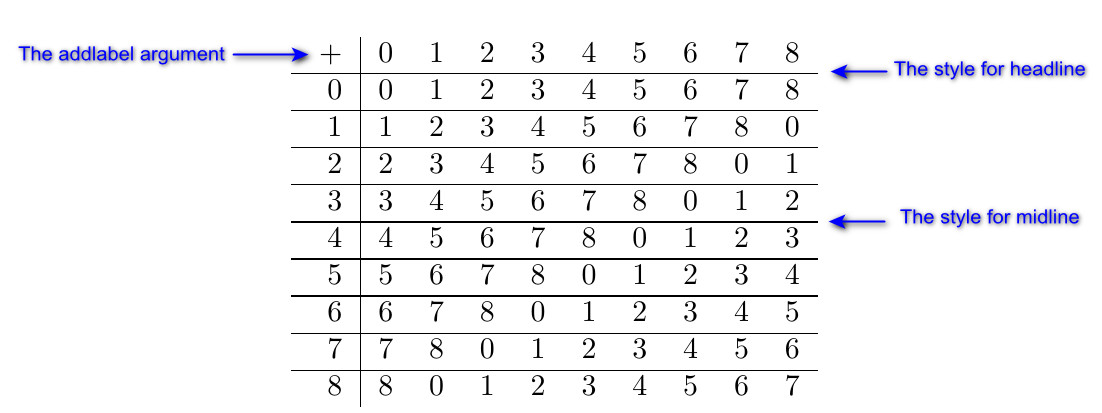
\includegraphics[scale=0.27]{luamodularadd.jpg}
  \caption{Optional arguments in luaModularAdd command}
  \label{fig:luamodularadd}
\end{figure}
\subsubsection{Illustration of luaModularAdd command }
This section illustrates the use of \verb|\luaModularAdd| command with several examples.
\begin{lstlisting}[caption={Illustration 1 of luaModularAdd command} ,label={luamodadd1}]
\begin{tabular}{r|rrrrrrrrr}
\luaModularAdd{9}
\end{tabular}
\end{lstlisting}

The LaTeX code in listing \ref{luamodadd1} generates the output shown in Table  \ref{luamodadd1tbl}.
\begin{table}[H]
\centering
\begin{tabular}{r|rrrrrrrrr}
$+$ & $0$ & $1$ & $2$ & $3$ & $4$ & $5$ & $6$ & $7$ & $8$\\ $0$ & $0$ & $1$ & $2$ & $3$ & $4$ & $5$ & $6$ & $7$ & $8$\\ $1$ & $1$ & $2$ & $3$ & $4$ & $5$ & $6$ & $7$ & $8$ & $0$\\ $2$ & $2$ & $3$ & $4$ & $5$ & $6$ & $7$ & $8$ & $0$ & $1$\\ $3$ & $3$ & $4$ & $5$ & $6$ & $7$ & $8$ & $0$ & $1$ & $2$\\ $4$ & $4$ & $5$ & $6$ & $7$ & $8$ & $0$ & $1$ & $2$ & $3$\\ $5$ & $5$ & $6$ & $7$ & $8$ & $0$ & $1$ & $2$ & $3$ & $4$\\ $6$ & $6$ & $7$ & $8$ & $0$ & $1$ & $2$ & $3$ & $4$ & $5$\\ $7$ & $7$ & $8$ & $0$ & $1$ & $2$ & $3$ & $4$ & $5$ & $6$\\ $8$ & $8$ & $0$ & $1$ & $2$ & $3$ & $4$ & $5$ & $6$ & $7$
\end{tabular}
\caption{Illustration 1 of luaModularAdd command}
\label{luamodadd1tbl}
\end{table}


The following code is generated by the command \verb|\luaModularAdd{9}|.
\begin{lstlisting}
$+$ & $0$ & $1$ & $2$ & $3$ & $4$ & $5$ & $6$ & $7$ & $8$\\
$0$ & $0$ & $1$ & $2$ & $3$ & $4$ & $5$ & $6$ & $7$ & $8$\\
$1$ & $1$ & $2$ & $3$ & $4$ & $5$ & $6$ & $7$ & $8$ & $0$\\
$2$ & $2$ & $3$ & $4$ & $5$ & $6$ & $7$ & $8$ & $0$ & $1$\\
$3$ & $3$ & $4$ & $5$ & $6$ & $7$ & $8$ & $0$ & $1$ & $2$\\
$4$ & $4$ & $5$ & $6$ & $7$ & $8$ & $0$ & $1$ & $2$ & $3$\\
$5$ & $5$ & $6$ & $7$ & $8$ & $0$ & $1$ & $2$ & $3$ & $4$\\
 $6$ & $6$ & $7$ & $8$ & $0$ & $1$ & $2$ & $3$ & $4$ & $5$\\
 $7$ & $7$ & $8$ & $0$ & $1$ & $2$ & $3$ & $4$ & $5$ & $6$\\
$8$ & $8$ & $0$ & $1$ & $2$ & $3$ & $4$ & $5$ & $6$ & $7$
\end{lstlisting}
Let us see some more examples of \verb|\luaModularAdd| command with optional arguments.
\begin{lstlisting}[caption={Illustration 2 of luaModularAdd command} ,label={luamodadd2}]
\begin{tabular}{r|rrrrrrrrr}
\luaModularAdd[headline=\hline]{9}
\end{tabular}
\end{lstlisting}
The LaTeX code in listing \ref{luamodadd2} generates the output shown in Table  \ref{luamodadd2tbl}. Here the style of \verb|headline| is specified as \verb|\hline|.

\begin{table}[H]
\centering
\begin{tabular}{r|rrrrrrrrr}
$+$ & $0$ & $1$ & $2$ & $3$ & $4$ & $5$ & $6$ & $7$ & $8$\\ \hline $0$ & $0$ & $1$ & $2$ & $3$ & $4$ & $5$ & $6$ & $7$ & $8$\\ $1$ & $1$ & $2$ & $3$ & $4$ & $5$ & $6$ & $7$ & $8$ & $0$\\ $2$ & $2$ & $3$ & $4$ & $5$ & $6$ & $7$ & $8$ & $0$ & $1$\\ $3$ & $3$ & $4$ & $5$ & $6$ & $7$ & $8$ & $0$ & $1$ & $2$\\ $4$ & $4$ & $5$ & $6$ & $7$ & $8$ & $0$ & $1$ & $2$ & $3$\\ $5$ & $5$ & $6$ & $7$ & $8$ & $0$ & $1$ & $2$ & $3$ & $4$\\ $6$ & $6$ & $7$ & $8$ & $0$ & $1$ & $2$ & $3$ & $4$ & $5$\\ $7$ & $7$ & $8$ & $0$ & $1$ & $2$ & $3$ & $4$ & $5$ & $6$\\ $8$ & $8$ & $0$ & $1$ & $2$ & $3$ & $4$ & $5$ & $6$ & $7$
\end{tabular}
\caption{Illustration 2 of luaModularAdd command}
\label{luamodadd2tbl}
\end{table}

\begin{lstlisting}[caption={Illustration 3 of luaModularAdd command} ,label={luamodadd3}]
\begin{tabular}{r|rrrrrrrrr}
\luaModularAdd[headline=\hline,
midline=\hline]{9}
\end{tabular}
\end{lstlisting}
The LaTeX code in listing \ref{luamodadd3} generates the output shown in Table  \ref{luamodadd3tbl}. Here the style of the \verb|headline| and \verb|midline| is specified as \verb|\hline|.

\begin{table}[H]
\centering
\begin{tabular}{r|rrrrrrrrr}
$+$ & $0$ & $1$ & $2$ & $3$ & $4$ & $5$ & $6$ & $7$ & $8$\\ \hline $0$ & $0$ & $1$ & $2$ & $3$ & $4$ & $5$ & $6$ & $7$ & $8$\\ \hline $1$ & $1$ & $2$ & $3$ & $4$ & $5$ & $6$ & $7$ & $8$ & $0$\\ \hline $2$ & $2$ & $3$ & $4$ & $5$ & $6$ & $7$ & $8$ & $0$ & $1$\\ \hline $3$ & $3$ & $4$ & $5$ & $6$ & $7$ & $8$ & $0$ & $1$ & $2$\\ \hline $4$ & $4$ & $5$ & $6$ & $7$ & $8$ & $0$ & $1$ & $2$ & $3$\\ \hline $5$ & $5$ & $6$ & $7$ & $8$ & $0$ & $1$ & $2$ & $3$ & $4$\\ \hline $6$ & $6$ & $7$ & $8$ & $0$ & $1$ & $2$ & $3$ & $4$ & $5$\\ \hline $7$ & $7$ & $8$ & $0$ & $1$ & $2$ & $3$ & $4$ & $5$ & $6$\\ \hline $8$ & $8$ & $0$ & $1$ & $2$ & $3$ & $4$ & $5$ & $6$ & $7$
\end{tabular}
\caption{Illustration 3 of luaModularAdd command}
\label{luamodadd3tbl}
\end{table}

In the following example, the formatting of the top line (before the beginning of the first row) and bottom line (after the end of the last row) are given in TeX document explicitly, and the style of the \verb|headline| and \verb|midline| is specified as \verb|\hline| through optional arguments of the command \verb|\luaModularAdd|.
\begin{lstlisting}[caption={Illustration 4 of luaModularAdd command} ,label={luamodadd4}]
\begin{tabular}{r|rrrrrrrrr}
\hline
\luaModularMult[headline=\hline]{9} \\
\hline
\end{tabular}
\end{lstlisting}
The LaTeX code in listing \ref{luamodadd4} generates the output shown in Table  \ref{luamodadd4tbl}.
\begin{table}[H]
\centering
\begin{tabular}{r|rrrrrrrrr}
\hline
$+$ & $0$ & $1$ & $2$ & $3$ & $4$ & $5$ & $6$ & $7$ & $8$\\
\hline $0$ & $0$ & $1$ & $2$ & $3$ & $4$ & $5$ & $6$ & $7$ & $8$\\
 $1$ & $1$ & $2$ & $3$ & $4$ & $5$ & $6$ & $7$ & $8$ & $0$\\
 $2$ & $2$ & $3$ & $4$ & $5$ & $6$ & $7$ & $8$ & $0$ & $1$\\
 $3$ & $3$ & $4$ & $5$ & $6$ & $7$ & $8$ & $0$ & $1$ & $2$\\
$4$ & $4$ & $5$ & $6$ & $7$ & $8$ & $0$ & $1$ & $2$ & $3$\\
$5$ & $5$ & $6$ & $7$ & $8$ & $0$ & $1$ & $2$ & $3$ & $4$\\
$6$ & $6$ & $7$ & $8$ & $0$ & $1$ & $2$ & $3$ & $4$ & $5$\\
 $7$ & $7$ & $8$ & $0$ & $1$ & $2$ & $3$ & $4$ & $5$ & $6$\\
$8$ & $8$ & $0$ & $1$ & $2$ & $3$ & $4$ & $5$ & $6$ & $7$ \\
\hline
\end{tabular} 
\caption{Illustration 4 of luaModularAdd command}
\label{luamodadd4tbl}
\end{table}

The \verb|booktabs| package can be used for beautifying tables. The following piece of code illustrates this.
\begin{lstlisting}[caption={Illustration 5 of luaModularAdd command} ,label={luamodadd5}]
\begin{tabular}{r|rrrrrrrrr}
\toprule
\luaModularAdd[headline=\midrule]{9} \\
\bottomrule
\end{tabular}
\end{lstlisting}
The LaTeX code in listing \ref{luamodadd5} generates the output shown in Table  \ref{luamodadd5tbl}.

\begin{table}[H]
\centering
\begin{tabular}{r|rrrrrrrrr}
\toprule
$+$ & $0$ & $1$ & $2$ & $3$ & $4$ & $5$ & $6$ & $7$ & $8$\\ \midrule $0$ & $0$ & $1$ & $2$ & $3$ & $4$ & $5$ & $6$ & $7$ & $8$\\ $1$ & $1$ & $2$ & $3$ & $4$ & $5$ & $6$ & $7$ & $8$ & $0$\\ $2$ & $2$ & $3$ & $4$ & $5$ & $6$ & $7$ & $8$ & $0$ & $1$\\ $3$ & $3$ & $4$ & $5$ & $6$ & $7$ & $8$ & $0$ & $1$ & $2$\\ $4$ & $4$ & $5$ & $6$ & $7$ & $8$ & $0$ & $1$ & $2$ & $3$\\ $5$ & $5$ & $6$ & $7$ & $8$ & $0$ & $1$ & $2$ & $3$ & $4$\\ $6$ & $6$ & $7$ & $8$ & $0$ & $1$ & $2$ & $3$ & $4$ & $5$\\ $7$ & $7$ & $8$ & $0$ & $1$ & $2$ & $3$ & $4$ & $5$ & $6$\\ $8$ & $8$ & $0$ & $1$ & $2$ & $3$ & $4$ & $5$ & $6$ & $7$ \\
\bottomrule
\end{tabular} 
\caption{Illustration 5 of luaModularAdd command}
\label{luamodadd5tbl}
\end{table}

As the last illustration, the optional parameter \verb|addlabel| is specified  in  \verb|\luaModularAdd| command.  If  a more complex expression (especially involving  a comma) is to be entered, it is better to enclose the code in curly braces as in the following example. The same rule  applies to other keys as well. This needs the \verb|amsmath| and \verb|amssymb| package for successful compilation.
\begin{lstlisting}[caption={Illustration 6 of luaModularAdd command} ,label={luamodadd6}]
\begin{tabular}{r|rrrrrrrrr}
\toprule
\luaModularAdd[addlabel={$(\mathbb{Z}_9,+)$},headline=\midrule]{9} \\
\bottomrule
\end{tabular}
\end{lstlisting}
The LaTeX code in listing \ref{luamodadd6} generates the output shown in Table  \ref{luamodadd6tbl}.
\begin{table}[H]
\centering
\begin{tabular}{r|rrrrrrrrr}
\toprule
$\mathbb{Z}_9$  & $0$ & $1$ & $2$ & $3$ & $4$ & $5$ & $6$ & $7$ & $8$\\ \midrule $0$ & $0$ & $1$ & $2$ & $3$ & $4$ & $5$ & $6$ & $7$ & $8$\\ $1$ & $1$ & $2$ & $3$ & $4$ & $5$ & $6$ & $7$ & $8$ & $0$\\ $2$ & $2$ & $3$ & $4$ & $5$ & $6$ & $7$ & $8$ & $0$ & $1$\\ $3$ & $3$ & $4$ & $5$ & $6$ & $7$ & $8$ & $0$ & $1$ & $2$\\ $4$ & $4$ & $5$ & $6$ & $7$ & $8$ & $0$ & $1$ & $2$ & $3$\\ $5$ & $5$ & $6$ & $7$ & $8$ & $0$ & $1$ & $2$ & $3$ & $4$\\ $6$ & $6$ & $7$ & $8$ & $0$ & $1$ & $2$ & $3$ & $4$ & $5$\\ $7$ & $7$ & $8$ & $0$ & $1$ & $2$ & $3$ & $4$ & $5$ & $6$\\ $8$ & $8$ & $0$ & $1$ & $2$ & $3$ & $4$ & $5$ & $6$ & $7$ \\
\bottomrule
\end{tabular}
\caption{Illustration 6 of luaModularAdd command}
\label{luamodadd6tbl}
\end{table}

\printbibliography
\end{document}
